\documentclass[UTF8]{ctexart}

\usepackage[a4paper,margin=2.5cm]{geometry}
\usepackage{booktabs}
\usepackage{graphicx}
\usepackage{hyperref}
\usepackage{float}
\usepackage{enumitem}
\usepackage{amsmath}
\usepackage{amssymb}

\graphicspath{
  {../../../units/assignment2/results/baseline/figures/}
  {../../../units/assignment2/results/hparam_tuning/conv_learning_rate_search_20260601_215042/}
  {../../../units/assignment2/results/hparam_tuning/conv_capacity_reg_search_20260601_223059/}
  {../../../units/assignment2/results/ablation/fc_normalization_dropout_ablation_20260601_210225/}
  {../../../units/assignment2/results/ablation/conv_regularization_ablation_20260601_211157/}
}

\title{第 2 周学习报告：CS231n Assignment 2}
\author{WalkerZJH}
\date{2026.05.25 -- 2026.05.30}

\begin{document}

\maketitle

\section{任务背景与目标}

本阶段围绕 CS231n Assignment 2 展开，主题包括归一化、dropout、卷积网络、优化器和 PyTorch RNN/LSTM captioning 前向路径。该任务的核心目标是在 NumPy 代码中手写 forward/backward，通过可复现实验理解网络层、梯度传播、训练稳定性和泛化之间的关系。

本报告将当前阶段目标分为三类：
\begin{itemize}
  \item \textbf{实现目标}：补全 Batch Normalization、Layer Normalization、Dropout、Convolution、Pooling、Spatial BatchNorm、GroupNorm、优化器、FullyConnectedNet、ThreeLayerConvNet 以及 PyTorch captioning 前向路径。
  \item \textbf{验证目标}：通过 shape 检查、数值梯度检查、小数据过拟合测试和训练曲线 sanity check 验证核心实现是否可靠。
  \item \textbf{探索目标}：围绕学习率、初始化、归一化、dropout、卷积结构、正则化和实现效率设计可复现的探索实验，用实验现象解释模型训练行为。
\end{itemize}

当前代码、笔记和结果归档：
\begin{itemize}
  \item 过程代码：\texttt{units/assignment2/code/}；
  \item 学习笔记：\texttt{units/assignment2/notes/}；
  \item 实验设计：\texttt{units/assignment2/experiments/}；
  \item 实验结果：\texttt{units/assignment2/results/}；
  \item 阶段成果：\texttt{deliverables/week02\_assignment2/}。
\end{itemize}

\section{研究问题与探索路线}

本阶段围绕以下研究问题组织实现、验证和实验。

\begin{table}[H]
\centering
\begin{tabular}{p{0.14\linewidth}p{0.28\linewidth}p{0.30\linewidth}p{0.18\linewidth}}
\toprule
编号 & 研究问题 & 验证方法 & 观察指标 \\
\midrule
RQ1 & 自实现 forward/backward 是否正确 & shape 检查、数值梯度检查、小数据过拟合测试 & 相对误差、维度一致性、loss 是否下降 \\
RQ2 & 学习率、初始化、batch size 如何影响收敛 & 控制变量下的超参数搜索 & loss 曲线、收敛速度、震荡程度、验证准确率 \\
RQ3 & BatchNorm、Dropout、CNN 等模块如何影响稳定性和泛化 & 归一化/dropout 消融、MLP 与 CNN 对比、正则强度对比 & train/val/test accuracy、泛化差距、曲线稳定性 \\
RQ4 & naive 与向量化实现是否存在明显效率差异 & naive conv/pool 与快速路径计时对比 & 单次 forward/backward 时间、训练耗时 \\
\bottomrule
\end{tabular}
\caption{Assignment 2 的研究问题与验证路线}
\end{table}

后续章节按“实现机制 $\rightarrow$ 正确性验证 $\rightarrow$ 探索实验设计 $\rightarrow$ 结果分析”的顺序展开，避免只罗列结果。

\section{框架设计与实现}

\subsection{整体架构}

Assignment 2 的代码按功能拆分为四层：
\begin{itemize}
  \item \textbf{基础算子层}：\texttt{cs231n/layers.py} 实现 affine、ReLU、normalization、dropout、convolution、pooling 和 softmax loss。
  \item \textbf{优化器与训练层}：\texttt{cs231n/optim.py} 和 \texttt{cs231n/solver.py} 负责参数更新和训练循环。
  \item \textbf{模型层}：\texttt{cs231n/classifiers/fc\_net.py}、\texttt{cnn.py} 和 \texttt{rnn\_pytorch.py} 实现具体模型。
  \item \textbf{实验归档层}：\texttt{run\_assignment2\_experiments.py} 负责 baseline 复现，\texttt{run\_assignment2\_explorations.py} 负责后续探索 suite。
\end{itemize}

\subsection{模块接口设计}

核心层遵循统一接口：forward 返回输出和 cache，backward 接收上游梯度并利用 cache 计算输入梯度与参数梯度。这个设计把计算图中的局部信息保存在每个模块内部，使 loss、模型结构和优化器之间保持清晰边界。

\subsection{训练流程设计}

训练流程由模型、Solver 和优化器共同完成。模型负责参数初始化、forward/loss 和 backward；Solver 负责 mini-batch 采样、训练循环、准确率评估和学习率衰减；优化器只处理参数更新。BatchNorm 和 Dropout 依赖 train/test 模式，因此训练循环必须在不同阶段正确切换模式。

\section{核心模块原理与实现要点}

\subsection{Affine、ReLU 与 Softmax Cross Entropy}

Affine 层完成线性变换：
\[
out = xW + b
\]
反向传播中，$dx$、$dW$ 和 $db$ 分别来自矩阵乘法链式法则和 batch 维度求和。ReLU 提供非线性：
\[
out = \max(0, x), \quad dx = dout \cdot \mathbb{1}(x > 0)
\]
Softmax Cross Entropy 将分类 score 转为概率并计算平均负对数似然，同时向前一层提供初始梯度。它后续用于判断 loss 曲线是否正常下降。

\subsection{Batch Normalization 与 Layer Normalization}

Batch Normalization 在训练阶段对 batch 内每个特征统计均值和方差：
\[
\hat{x} = \frac{x-\mu}{\sqrt{\sigma^2+\epsilon}}, \quad y = \gamma \hat{x} + \beta
\]
并维护 running mean 与 running variance 供测试阶段使用。反向传播可按计算图逐步展开，也可合并为简化形式：
\[
dx =
\frac{1}{N}
\cdot
\frac{1}{\mathrm{std}}
\left(
N\,d\hat{x}
-
\sum d\hat{x}
-
\hat{x}\,\sum(d\hat{x}\odot\hat{x})
\right)
\]
Layer Normalization 的公式形式相同，但统计维度改为每个样本内部的特征维度，因此训练和测试阶段行为一致。

\subsection{Dropout}

当前实现使用 inverted dropout。训练阶段生成
\[
\operatorname{mask} = \frac{\operatorname{Bernoulli}(p)}{p}
\]
并令输出为 $x \odot \operatorname{mask}$；反向传播为
\[
dx = dout \odot \operatorname{mask}
\]
测试阶段直接返回输入。该模块后续用于分析随机屏蔽隐藏单元对泛化差距的影响。

\subsection{Convolution 与 Pooling}

卷积层利用局部感受野和参数共享提取图像空间模式。对输入 $x \in \mathbb{R}^{N \times C \times H \times W}$ 和滤波器 $w \in \mathbb{R}^{F \times C \times HH \times WW}$：
\[
\operatorname{out}_{n,f,i,j}
=
\sum
\left(
\operatorname{window}(x_n, i, j) \odot w_f
\right)
+ b_f
\]
naive 实现显式遍历样本、滤波器和空间位置，便于理解 padding、stride 和梯度累加；快速路径通过 im2col/col2im 将局部窗口转换为矩阵乘法，减少 Python 循环开销。

Max Pooling 在局部窗口中保留最大响应，backward 只将梯度传回 forward 中取得最大值的位置。该模块用于降低空间分辨率，并在 ThreeLayerConvNet 中控制特征图尺寸。

\subsection{Spatial BatchNorm 与 GroupNorm}

Spatial BatchNorm 将卷积特征图从 $(N,C,H,W)$ 变换为 $(N \cdot H \cdot W,C)$ 后复用普通 BatchNorm，对每个通道进行归一化。GroupNorm 将每个样本的通道拆为 $G$ 组，在组内统计均值和方差，不依赖 batch 统计，适合小 batch 或显存受限场景。

\subsection{PyTorch RNN/LSTM Captioning}

Captioning 模型中，图像特征先投影为初始 hidden state，caption token 经 embedding 后输入 RNN 或 LSTM，每个时间步的 hidden state 通过 temporal affine 得到词表 score，最后使用 masked temporal softmax 忽略 \texttt{<NULL>} padding。PyTorch 版本由 autograd 处理 backward，本阶段重点补全 forward 计算路径和采样流程。

\section{实验设置}

\subsection{数据集与划分}

当前正式 baseline 和探索实验均使用 CIFAR-10 完整训练设置：
\begin{itemize}
  \item 训练集：49000 张；
  \item 验证集：1000 张；
  \item 测试集：10000 张；
  \item 训练轮数：10 epochs；
  \item batch size：100；
\end{itemize}

\subsection{基础模型配置}

baseline 包含两类模型：
\begin{itemize}
  \item \textbf{FullyConnectedNet + BN + Dropout}：使用 Adam，学习率 $1e^{-3}$，隐藏层维度为 $[100,100]$，dropout keep ratio 为 0.8。
  \item \textbf{ThreeLayerConvNet}：使用 Adam，学习率 $1e^{-3}$，卷积核数量为 8，卷积核大小为 3。
\end{itemize}

\subsection{评价指标}

主要指标包括 train accuracy、validation accuracy、test accuracy、final loss 和 loss history。探索实验中额外关注 train-val gap、曲线震荡程度和单次训练耗时。

\subsection{控制变量原则}

每组探索实验只改变一个主要因素，例如学习率、初始化方式、是否加入 BatchNorm、是否加入 Dropout、正则强度或卷积网络容量；其余训练设置保持一致。这样结果才能用于解释具体因素对优化和泛化的影响。

\section{主动探索实验设计与运行结果}

\subsection{学习率搜索}

\begin{table}[H]
\centering
\begin{tabular}{ll}
\toprule
项目 & 内容 \\
\midrule
实验目的 & 观察学习率对下降速度、震荡程度和最终验证表现的影响。 \\
实验假设 & 学习率过大可能导致 loss 震荡或发散，过小则收敛缓慢。 \\
控制变量 & 固定模型结构、初始化、batch size、训练轮数和正则强度。 \\
对比设置 & ThreeLayerConvNet，$lr \in \{2\times10^{-3}, 10^{-3}, 5\times10^{-4}\}$。 \\
观察指标 & loss 曲线、train/val/test accuracy、final loss。 \\
\bottomrule
\end{tabular}
\caption{学习率搜索设计}
\end{table}

\subsection{归一化与 Dropout 消融}

FullyConnectedNet 消融固定隐藏层结构、优化器、学习率、正则强度、batch size 和训练轮数，只改变 normalization 与 dropout。该实验用于观察 BatchNorm、LayerNorm 和 Dropout 在当前浅层全连接网络中的实际作用。

\subsection{CNN 容量与 L2 正则探索}

ThreeLayerConvNet 探索分两组：一组只改变 L2 正则强度，用于分析正则项对 train-val gap 的影响；另一组同时比较卷积核数量、隐藏层维度和正则强度，用于观察容量提升是否能同步提升验证集表现。

\subsection{MLP 与 CNN 结构对比}

MLP 与 CNN 对比用于分析图像任务中空间结构的重要性。当前 baseline 包含 FullyConnectedNet + BN + Dropout 与 ThreeLayerConvNet；FC 消融还提供了无归一化、BatchNorm、LayerNorm 和 Dropout 的控制变量结果，使结构差异不只依赖单个全连接配置。

\subsection{Naive 与向量化实现效率对比}

效率观察来自  训练耗时：FullyConnectedNet 单个配置约 1.4--2.5 分钟，8-filter ThreeLayerConvNet 单个配置约 12--13 分钟，16-filter ThreeLayerConvNet 约 23.8 分钟。该现象说明卷积网络即使使用快速路径，训练仍明显受卷积层计算量影响。

\section{实验结果与分析}

\subsection{Baseline 结果}

\begin{table}[H]
\centering
\begin{tabular}{lrrrr}
\toprule
模型 & 训练准确率 & 验证准确率 & 测试准确率 & 最终 loss \\
\midrule
FullyConnectedNet + BN + Dropout & 0.3464 & 0.4010 & 0.3450 & 2.0812 \\
ThreeLayerConvNet & 0.7571 & 0.6110 & 0.6151 & 0.6619 \\
\bottomrule
\end{tabular}
\caption{CIFAR-10 完整训练设置 baseline 实验结果}
\end{table}

\begin{figure}[H]
\centering
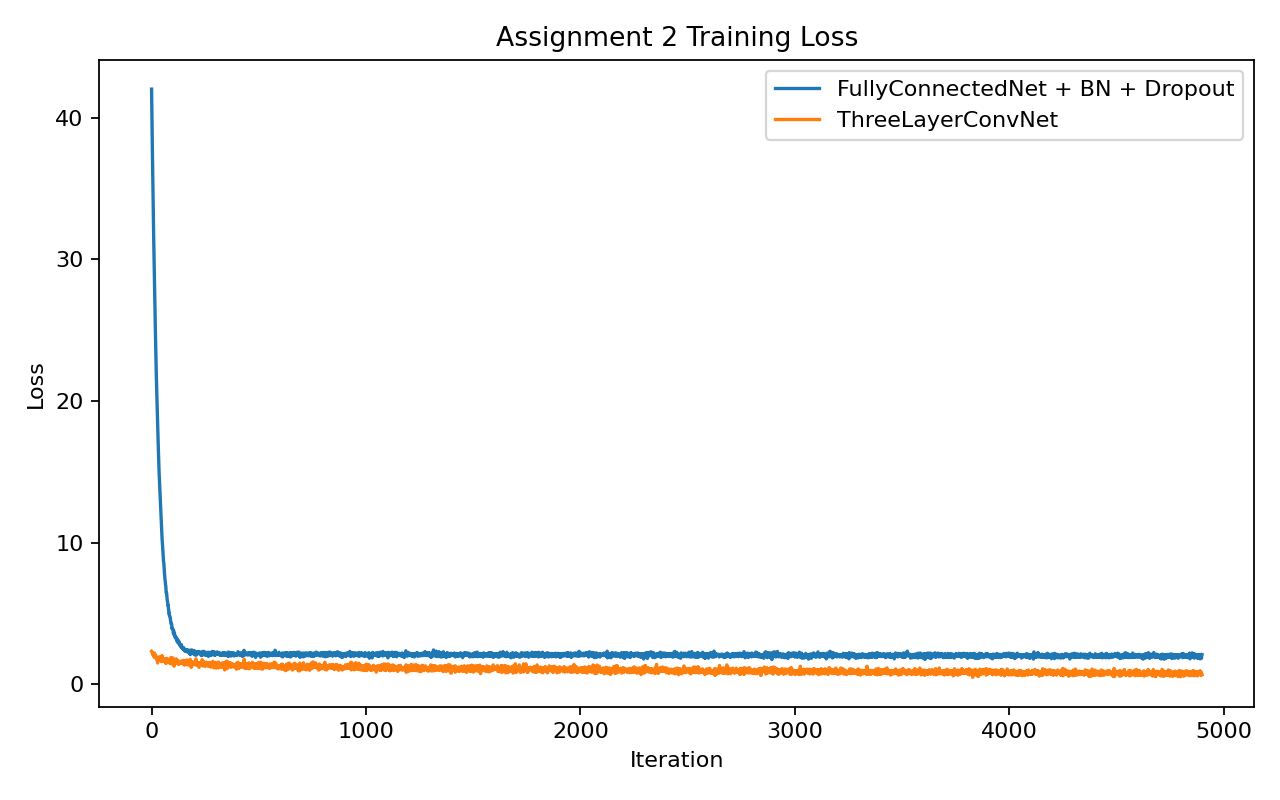
\includegraphics[width=0.82\linewidth]{assignment2_loss_curves.png}
\caption{Assignment 2 baseline 训练损失曲线}
\end{figure}

\begin{figure}[H]
\centering
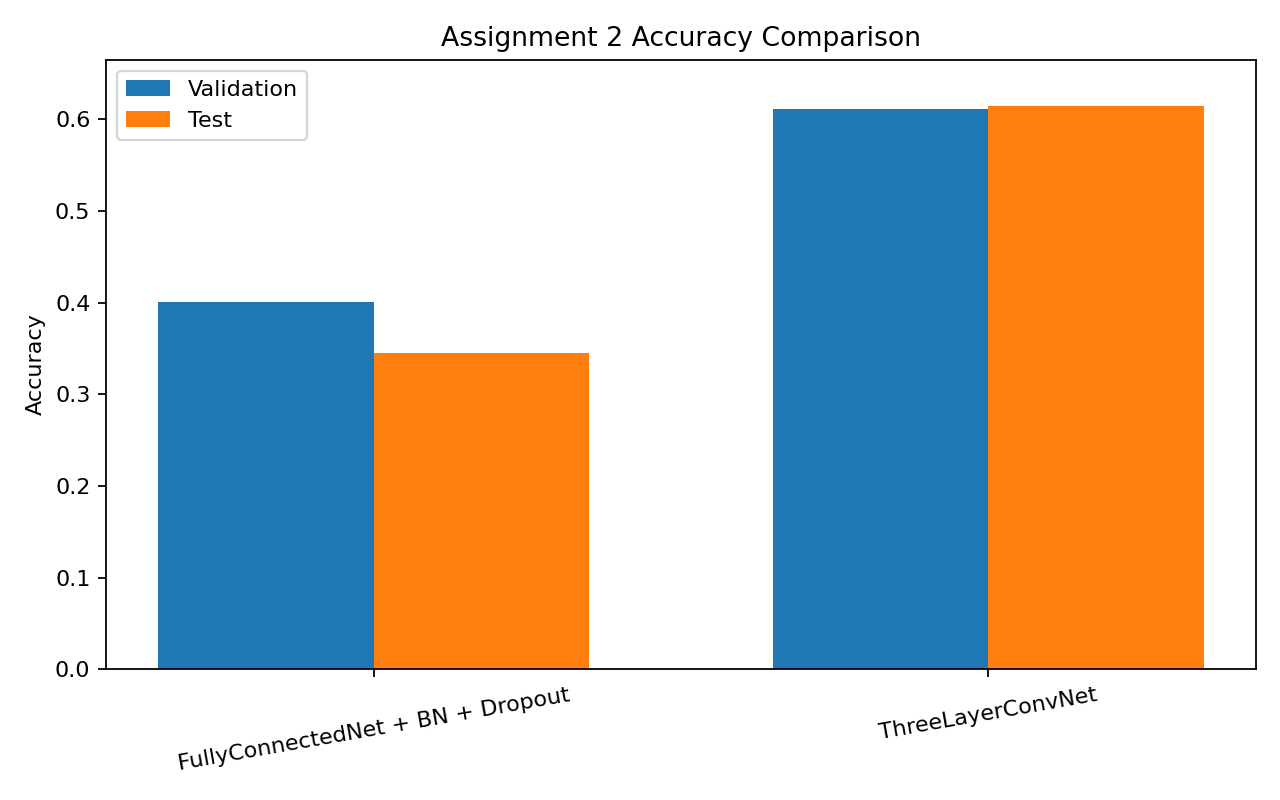
\includegraphics[width=0.82\linewidth]{assignment2_accuracy_comparison.png}
\caption{Assignment 2 baseline 验证集与测试集准确率对比}
\end{figure}

ThreeLayerConvNet 的测试准确率达到 0.6151，显著高于 FullyConnectedNet + BN + Dropout 的 0.3450。这符合图像任务中的基本预期：卷积层利用局部感受野和参数共享，更适合 CIFAR-10 这类具有空间结构的输入。与快速验证的小数据集表现相比，CNN 的测试表现明显提升，说明此前“训练集高、测试集低”的现象主要来自训练样本过少，而不是模型在完整数据设置下不可泛化。

\subsection{超参数搜索结果}

\begin{table}[H]
\centering
\begin{tabular}{lrrrrr}
\toprule
配置 & 学习率 & 训练准确率 & 验证准确率 & 测试准确率 & 最终 loss \\
\midrule
A2-HP-LR-001 & $2\times10^{-3}$ & 0.6593 & 0.5740 & 0.5768 & 0.8036 \\
A2-HP-LR-002 & $10^{-3}$ & 0.7572 & 0.6140 & 0.6006 & 0.6418 \\
A2-HP-LR-003 & $5\times10^{-4}$ & 0.7795 & 0.6020 & 0.6110 & 0.4926 \\
\bottomrule
\end{tabular}
\caption{ThreeLayerConvNet 学习率搜索结果}
\end{table}

学习率搜索中，$10^{-3}$ 的验证准确率最高，$5\times10^{-4}$ 的测试准确率略高但验证准确率低于 $10^{-3}$。按照验证集选择原则，当前学习率搜索选择 $10^{-3}$；同时记录 $5\times10^{-4}$ 的测试表现，说明较小学习率能进一步降低 loss，但不应直接用测试集反向选择超参数。

\begin{table}[H]
\centering
\begin{tabular}{lrrrrrr}
\toprule
配置 & filters & hidden & reg & 训练准确率 & 验证准确率 & 测试准确率 \\
\midrule
A2-HP-CNN-001 & 8 & 100 & $10^{-3}$ & 0.7572 & 0.6140 & 0.6006 \\
A2-HP-CNN-002 & 8 & 100 & $10^{-2}$ & 0.7012 & 0.6100 & 0.6157 \\
A2-HP-CNN-003 & 4 & 100 & $10^{-2}$ & 0.6604 & 0.5640 & 0.5651 \\
A2-HP-CNN-004 & 8 & 50 & $10^{-2}$ & 0.6969 & 0.6060 & 0.6159 \\
A2-HP-CNN-005 & 16 & 100 & $10^{-3}$ & 0.7791 & 0.6440 & 0.6350 \\
\bottomrule
\end{tabular}
\caption{ThreeLayerConvNet 容量与正则搜索结果}
\end{table}

\begin{figure}[H]
\centering
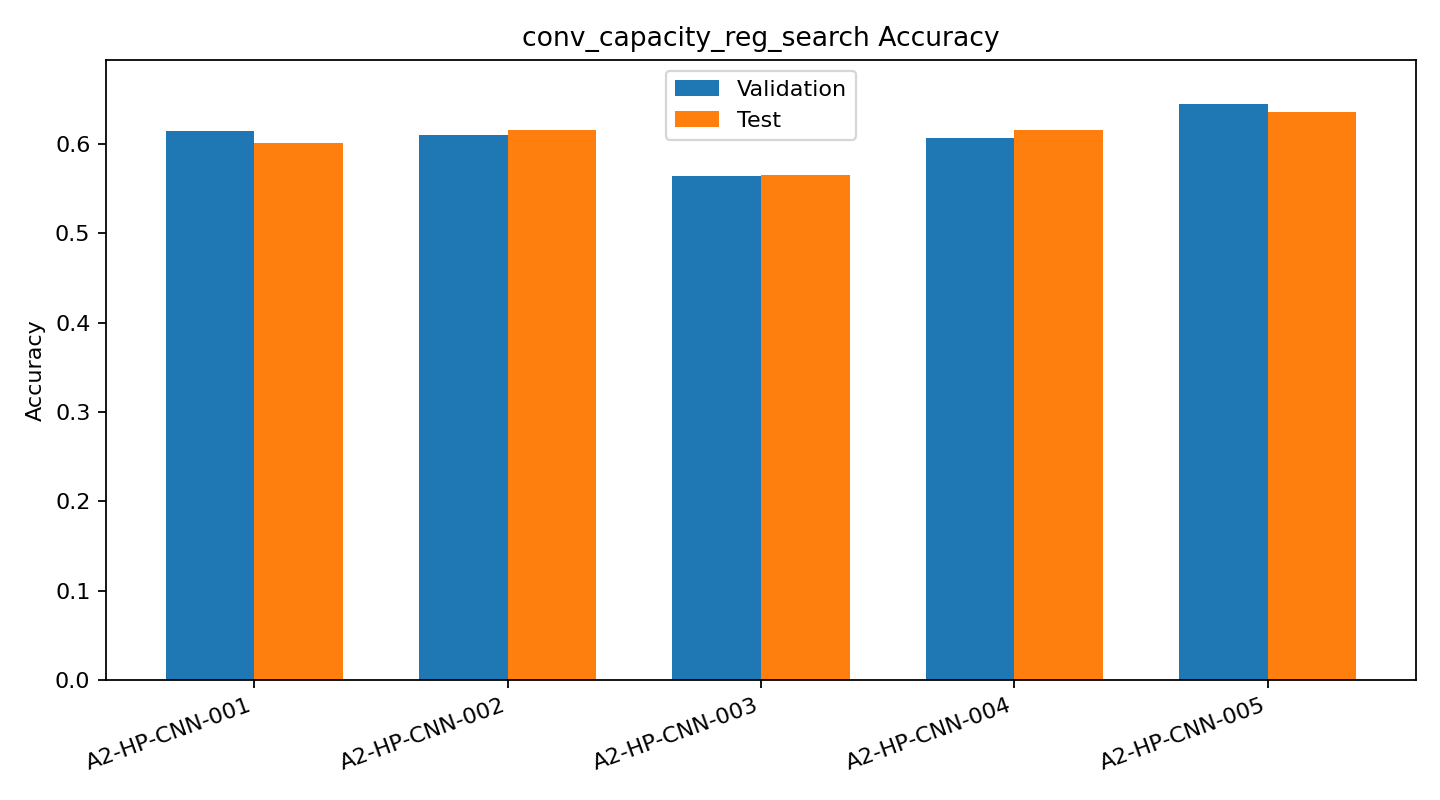
\includegraphics[width=0.82\linewidth]{conv_capacity_reg_search_accuracy.png}
\caption{ThreeLayerConvNet 容量与正则搜索准确率对比}
\end{figure}

容量搜索中，16 个卷积核的配置取得最高验证准确率 0.6440 和测试准确率 0.6350。降低卷积核数量到 4 会明显降低验证和测试表现；降低隐藏层维度到 50 后测试准确率接近强正则配置，但验证准确率没有超过 16-filter 配置。该结果说明在完整数据集下，适度增加卷积特征通道可以提升表示能力。

\subsection{模块消融结果}

\begin{table}[H]
\centering
\begin{tabular}{lrrrr}
\toprule
FC 配置 & 训练准确率 & 验证准确率 & 测试准确率 & train-val gap \\
\midrule
无归一化 / 无 Dropout & 0.4429 & 0.4420 & 0.4394 & 0.0009 \\
BatchNorm & 0.4138 & 0.4430 & 0.4118 & -0.0292 \\
LayerNorm & 0.4212 & 0.4380 & 0.4144 & -0.0168 \\
Dropout keep=0.8 & 0.2583 & 0.2870 & 0.2577 & -0.0287 \\
BatchNorm + Dropout keep=0.8 & 0.1726 & 0.2700 & 0.1728 & -0.0974 \\
\bottomrule
\end{tabular}
\caption{FullyConnectedNet 归一化与 Dropout 消融结果}
\end{table}

\begin{figure}[H]
\centering
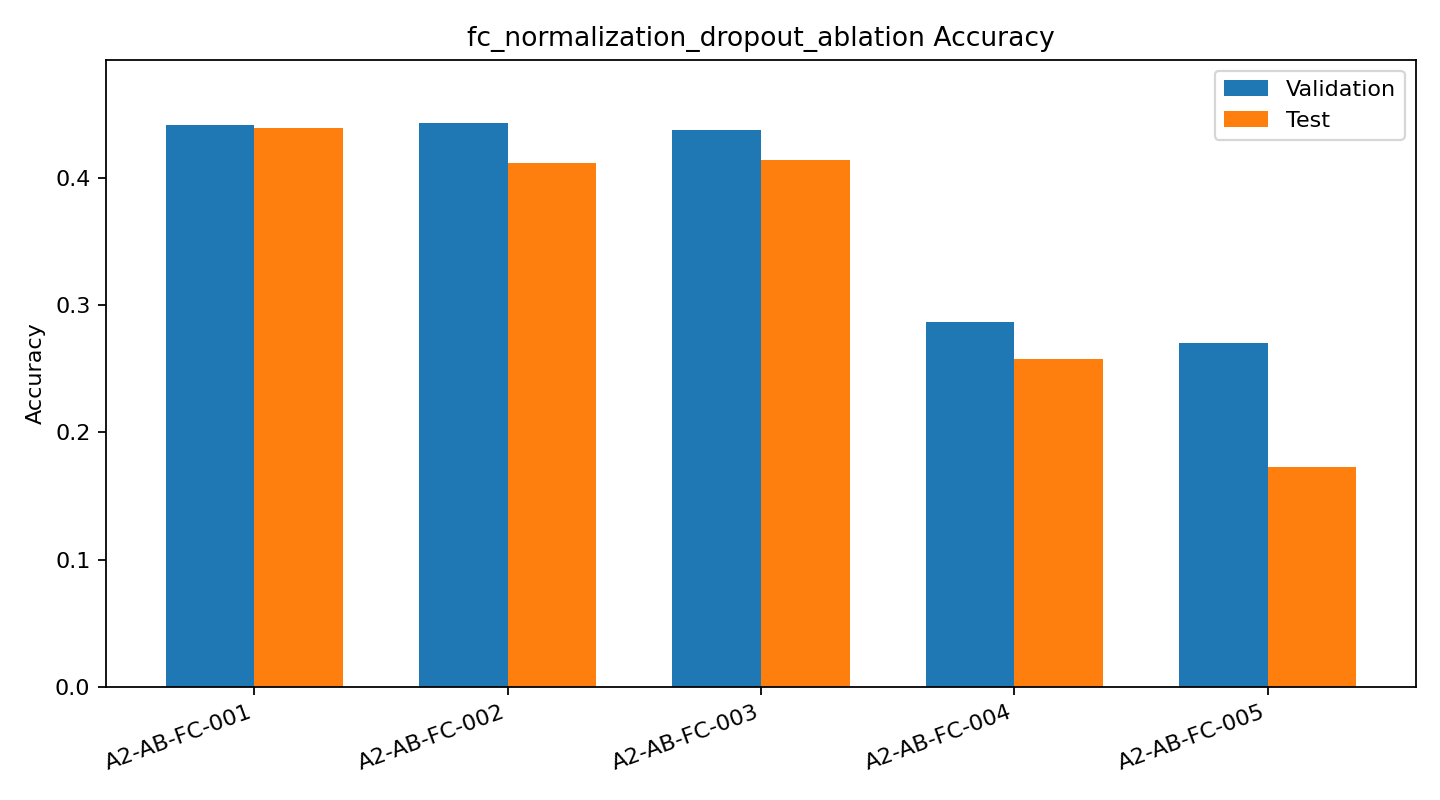
\includegraphics[width=0.82\linewidth]{fc_normalization_dropout_ablation_accuracy.png}
\caption{FullyConnectedNet 归一化与 Dropout 消融准确率对比}
\end{figure}

FC 消融显示，当前 10 epochs、浅层网络配置下，无归一化且不使用 Dropout 的测试准确率最高。BatchNorm 的验证准确率略高，但测试准确率低于无归一化配置；Dropout 及 BatchNorm+Dropout 明显降低训练和测试表现，说明当前模型容量和训练轮数下，随机屏蔽带来的欠拟合影响更强。

\begin{table}[H]
\centering
\begin{tabular}{lrrrr}
\toprule
CNN 配置 & 训练准确率 & 验证准确率 & 测试准确率 & train-val gap \\
\midrule
reg=$0$ & 0.7702 & 0.6140 & 0.6091 & 0.1562 \\
reg=$10^{-3}$ & 0.7572 & 0.6140 & 0.6006 & 0.1432 \\
reg=$10^{-2}$ & 0.7012 & 0.6100 & 0.6157 & 0.0912 \\
\bottomrule
\end{tabular}
\caption{ThreeLayerConvNet L2 正则消融结果}
\end{table}

CNN 正则消融中，增大 L2 正则会降低训练准确率并缩小 train-val gap。$reg=10^{-2}$ 的测试准确率略高，但验证准确率没有超过 $reg=0$ 与 $reg=10^{-3}$。该结果说明 L2 正则在当前训练设置下能一定程度上缓解过拟合，但它并不是提升验证准确率的必要条件。

\subsection{结构对比结果}

当前 baseline 中，FullyConnectedNet + BN + Dropout 的测试准确率为 0.3450，ThreeLayerConvNet 的测试准确率为 0.6151。即使将 FC 消融中的最佳测试配置纳入比较，无归一化 FC 的测试准确率也只有 0.4394，仍明显低于 CNN。这说明卷积结构对图像空间结构的利用是 Assignment 2 中最关键的性能来源。

\subsection{效率对比结果}

从运行 trace 看，FC 单个配置耗时约 83--151 秒；8-filter CNN 单个配置约 740--776 秒；16-filter CNN 单个配置约 1427 秒。CNN 容量提升带来更高准确率，也显著增加训练耗时。

\section{问题、调试过程与解决方案}


\subsection{loss 不下降的定位}

loss 不下降时优先检查学习率、初始化尺度、梯度符号、正则项、数据预处理和 train/test 模式。本阶段的学习率搜索和正则消融都保留了 loss history，可用于定位训练震荡、欠拟合或容量不足。

\subsection{过拟合与正则化选择}

早期快速验证口径下，ThreeLayerConvNet 出现训练准确率高而测试准确率低的现象。full-data baseline 将测试准确率提升到 0.6151，容量搜索进一步提升到 0.6350，说明主要问题来自训练样本过少。当前完整训练设置下仍有约 0.13--0.15 的 train-val gap，但它已经不再表现为严重泛化不足。

\section{阶段性总结与后续计划}

\subsection{本阶段完成内容}

本阶段完成了 Assignment 2 的核心实现、 baseline、CNN 学习率搜索、CNN 容量/正则搜索、FC 归一化/Dropout 消融和 CNN L2 正则消融。实验结果已保存为 CSV、JSON、运行 trace 和可视化图。

\subsection{模型理解方面的收获}

通过手写 forward/backward，当前阶段建立了对 cache、局部梯度、loss 初始梯度、train/test 模式和卷积窗口梯度累加的整体理解。Baseline 结果也说明，图像任务中卷积结构对空间信息的利用明显优于直接展开输入的全连接结构。

\end{document}
